\documentclass{article}

\usepackage{graphicx}
\usepackage{tikz}
\usepackage{tikzsymbols}
\usetikzlibrary{calc,patterns,shapes.geometric}
\pagestyle{empty}
\usepackage[margin=0pt]{geometry}
\geometry{papersize={14in,12in}}

\def\centerarc[#1](#2)(#3:#4:#5){\draw[#1] ($(#2)+({#5*cos(#3)},{#5*sin(#3)})$) arc (#3:#4:#5);}

\begin{document}
	\begin{figure}
		\centering
		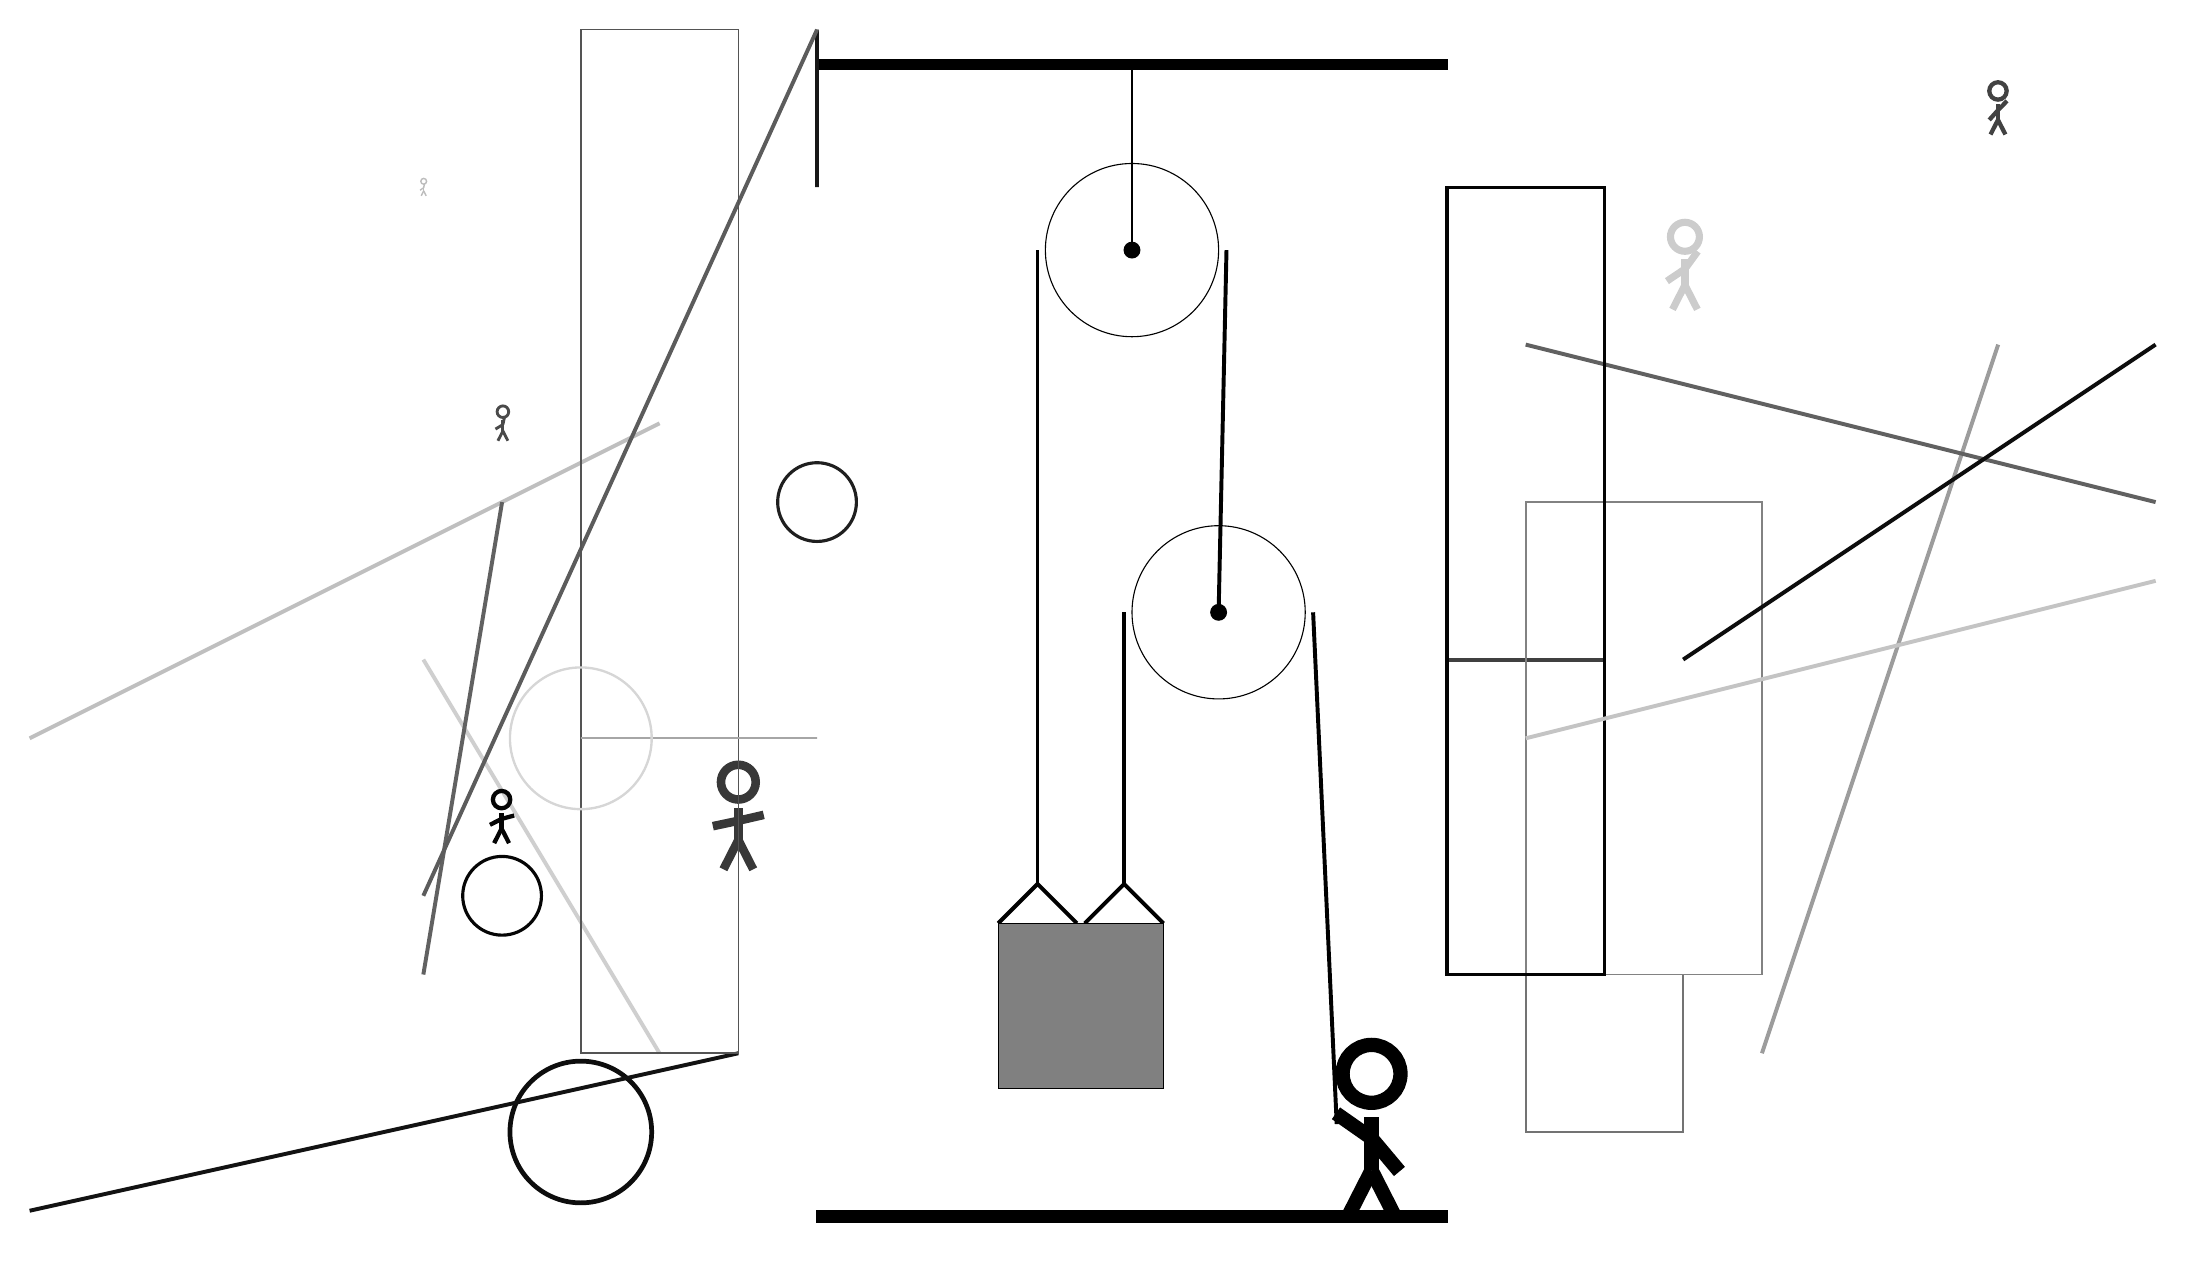
\begin{tikzpicture}
			%%%%% START %%%%%
			
			\draw[fill=black] (-2, 11.5) rectangle (6, 11.625);
			
			\draw (2, 9.2) circle (1.1);
			\draw[fill=black] (2, 9.2) circle (0.1);
			\draw[thick] (2, 9.2) -- (2, 11.5);
			
			\draw (3.1, 4.6) circle (1.1);
			\draw[fill=black] (3.1, 4.6) circle (0.1);
			
			\draw[line width = 0.5mm]  (0.3, 0.65) -- (0.8, 1.15) -- (1.3, 0.65);
			\draw[line width = 0.5mm]  (1.4, 0.65) -- (1.9, 1.15) -- (2.4, 0.65);
			\draw[fill=black!50] (0.3, 0.65) rectangle (2.4, -1.45);
			
			\draw[line width = 0.5mm] (0.8, 9.2) -- (0.8, 1.15);
			\centerarc[line width = 0.5mm](2, 9.2)(0:180:1.2000000000000002);
			\draw[line width = 0.5mm] (3.2, 9.2) -- (3.1, 4.6);
			\draw[line width = 0.5mm] (1.9, 4.6) -- (1.9, 1.15);
			\centerarc[line width = 0.5mm](3.1, 4.6)(0:180:1.2000000000000002);
			\draw[line width = 0.5mm] (4.3, 4.6) -- (4.6, -1.9);
			
			\node at (5, -2) {\Strichmaxerl[10][-35][-50]};
			
			\draw[line width=0.5mm, color=black!39](10, -1) -- (13, 8);
			
			\draw[line width=0.5mm, color=black!19](-7, 4) -- (-4, -1);
			\draw[line width=0.5mm, color=black!75] (6, 4) rectangle (8, 4);
			\draw[line width=0.5mm, color=black!91] (-2, 12) rectangle (-2, 10);
			
			\draw [line width=0.6mm, color=black!95](-5, -2) circle (0.9);
			\draw [line width=0.4mm, color=black!88](-2, 6) circle (0.5);
			\draw[line width=0.5mm, color=black!62](7, 8) -- (15, 6);
			\node[line width=0.6mm, color=black!74] at (13, 11) {\Strichmaxerl[3][48][46]};
			\draw[line width=0.5mm, color=black!25](-4, 7) -- (-12, 3);
			\node[line width=0.5mm, color=black!98] at (-6, 2) {\Strichmaxerl[3][27][15]};
			
			\draw [line width=0.3mm, color=black!65](-9, 5) circle (0.0);
			\draw[line width=0.2mm, color=black!55] (7, -2) rectangle (9, 0);
			\draw[line width=0.5mm, color=black!93](-3, -1) -- (-12, -3);
			
			\draw[line width=0.2mm, color=black!49] (7, 6) rectangle (10, 0);
			\draw[line width=0.5mm, color=black!62](-6, 6) -- (-7, 0);
			\node[line width=0.3mm, color=black!78] at (-3, 2) {\Strichmaxerl[6][12][13]};
			
			\node[line width=0.2mm, color=black!26] at (-7, 10) {\Strichmaxerl[1][34][78]};
			\draw[line width=0.5mm, color=black!95](9, 4) -- (15, 8);
			\node[line width=0.7mm, color=black!20] at (9, 9) {\Strichmaxerl[5][34][54]};
			\draw[line width=0.5mm, color=black!64](-2, 12) -- (-7, 1);
			\draw[line width=0.4mm, color=black!99] (8, 0) rectangle (6, 10);
			
			\draw [line width=0.4mm, color=black!98](-6, 1) circle (0.5);
			
			\draw[line width=0.2mm, color=black!67] (-3, -1) rectangle (-5, 12);
			\draw[line width=0.5mm, color=black!23](7, 3) -- (15, 5);
			\draw[line width=0.3mm, color=black!35] (-2, 3) rectangle (-5, 3);
			\draw [line width=0.3mm, color=black!16](-5, 3) circle (0.9);
			\node[line width=0.2mm, color=black!71] at (-6, 7) {\Strichmaxerl[2][31][78]};
			
			\draw[fill=black] (-2, -3) rectangle (6, -3.15);
			
			%%%%% END %%%%%
		\end{tikzpicture}
	\end{figure}	
\end{document}